%%%%%%%%%%%%%%%%%%%%%%%%%%%%POSTER%%%%%%%%%%%%%%%%%%%%%%%%%%%%%%
\block{Introdução}{
	As balanças foram criadas por necessidade durante o desenvolvimento de comercio na antiguidade, os produtos que não recorriam a contagem por unidades, tais como objetos irregulares por exemplo o ouro tinham de se quantificar seu valor, e a forma de medir sua massa tornou-se numa variável de medição para troca de bens. As primeiras balanças eram alavancas em equilíbrio [ F1 × b1c = F2 × b2c ], onde nos extremos eram colocados cestos e se colocava os pesos, este estava centrado no seu centro de massa, assim se os pesos nos dois cestos serem iguais fica em equilíbrio, era um sistema de comparar com pesos fixos estabelecidos como norma (contra-pesos).\\
	Os métodos de medir a massa de objetos não conheceu nenhumas melhorias tecnológicas relevantes até a era industrial. Só nos anos do século XVIII é que o meio de medir a massa de objetos não dependia de contra-pesos. As balanças por molas foi inventado por Richard Salter, um fabricante de balanças por volta dos anos de 1770 na Inglaterra.\\
	O que vai ser utilizado no projeto vai ser um \textbf{célula de peso}, estas células tem quatro sensores \textit{strain gauges} ligadas em ponte wheatstone que vão detetar a distorção (pressão) do material, ou seja, a célula de peso e gerar um sinal em tensão proporcional a força exercida quando alimentado. Seque o mesmo principio de uma mola [ $K= \frac{\Delta l}{F}$ ].
}
\begin{columns}
\column{0.1}
\column{0.8}
\block{Kit Desenvolvimento}{
	\begin{tikzfigure}
		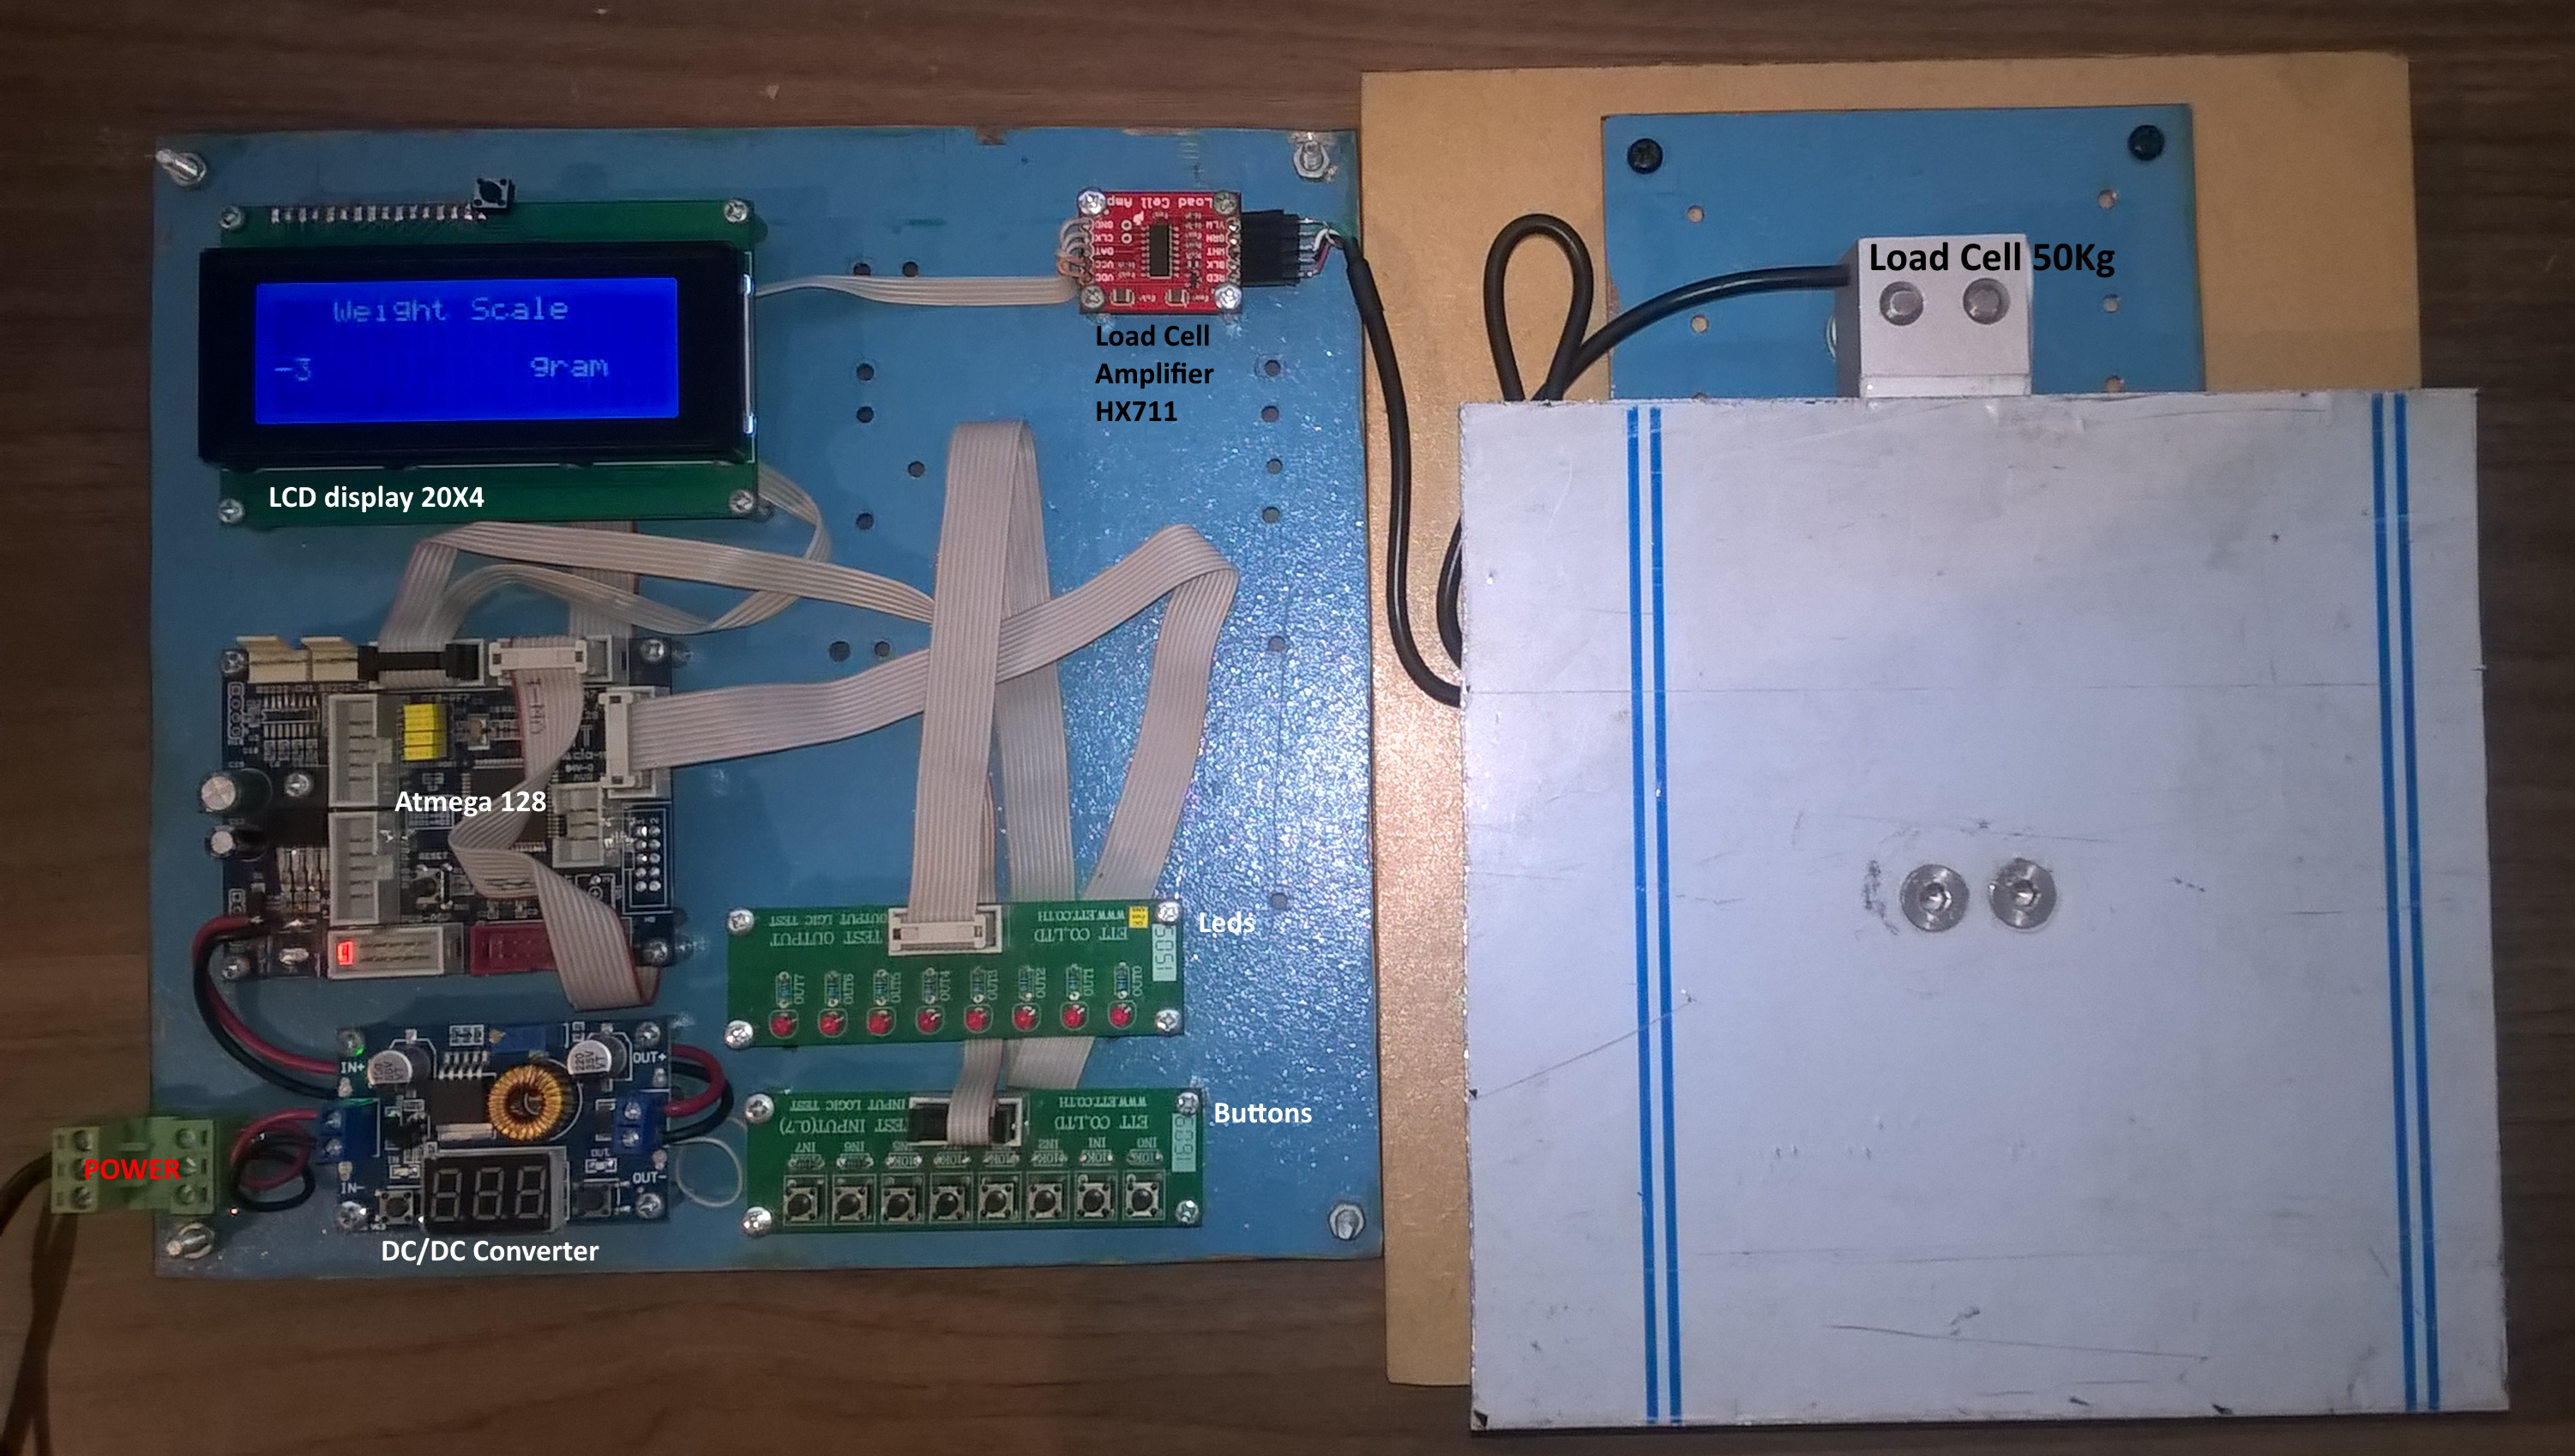
\includegraphics[width=0.7\textwidth]{./image/PESTA/kit/Kit_Desenvolvimento_2.jpg}
	\end{tikzfigure}
}
\end{columns}
\begin{columns}
\column{0.5}
\block{Sensor}{
	O sensor é um transdutor utilizado em converter energia de uma natureza para outra como entrada de sinal para um sistema, são os elementos principais de interface com o mundo real para o analógico. \\
	Neste projecto é o caso de utilizar uma celula de peso, ou seja, sensores piezoresistivos para determinar a massa dos objectos.
	
}
\column{0.5}
\block{Informação e Controlo}{
	Paragraph \vspace{.1cm}
	
}
\end{columns}
\begin{columns}
\column{1}
\block{More Examples of LateX}{
	\bigskip
	you can even put stuff in color boxes.\\
	\coloredbox{
		\begin{itemize}
			\item 1
			\item 2
		\end{itemize}
	}
	\bigskip
	\vspace{5cm}
}
\note[targetoffsetx=-34cm, targetoffsety=-4cm, width=.3\linewidth]{
	\texttt{https://github.com/sergio1020881/PESTA2021}
}
\end{columns}
%%%%%%%%%%%%%%%%%%%%%%%%%%%%%%%%%%%%%%%%%%%%%%%%%%%%%%%%%%%%%%%%
\begin{comment}
\begin{columns}
\column{.65}
\block{More Examples of LateX}{
	\bigskip
	you can even put stuff in color boxes.\\
	\coloredbox{
		\begin{itemize}
			\item 1
			\item 2
		\end{itemize}
		\lipsum[1]
		\bigskip
		\innerblock{LINK:}{
			\center
			https://github.com/sergio1020881/PESTA2021
		}
	}	
}
\block{More text}{
	\lipsum[1]
}
\column{.35}
\block{more pictures}{
	
\includegraphics[width=\linewidth]{./image/PESTA/ISEP_marca_cor_grande.png}
}
\block{the end}{
	\lipsum[1]
}
\block{referencces}{
%\printbibliography
}
\end{columns}
\end{comment}
%%%%%%%%%%%%%%%%%%%%%%%%%%%%%%%%%%%%%%%%%%%%%%%%%%%%%%%%%%%%%%%%